%
\documentclass[%
 reprint,
 amsmath,amssymb,
 aps,
]{revtex4-1}

\usepackage{graphicx}% Include figure files
\usepackage{dcolumn}% Align table columns on decimal point
\usepackage{bm}% bold math


\begin{document}


\title{Comparativa Metodologia Kimball vs Metodología Inmon}
\author{Robles Flores, Anthony Richard	               (2016056192)}
\author{Estrella Palacios, Katherine Lizbeth			(2015050948)}
\author{Sosa Bedoya, Sharon Fiorela					(2016054460)}
\author{Torres Beltran , Johanna Andrea				(2020067849)}

		
\affiliation{%
 Universidad Privada de Tacna \textbackslash Facultad de Ingenieria \textbackslash Escuela Profesional de Ingenieria de Sistemas
}%

\begin{abstract}
\begin{center}
\textbf{Resumen}
\end{center}
Los almacenes de datos (data warehouses en inglés) toman cada día mayor importancia, a medida que las organizaciones pasan de esquemas de sólo recolección de datos a esquemas de análisis de los mismos. En este breve artículo se  tratará de brindar una explicación general de algunas metodologías, en este caso serán la metodología Kimball y la metodología Inmon.
\\

\begin{center}
\textbf{Abstract}
\end{center}
Data warehouses (data warehouses in English) are becoming increasingly important, as organizations move from data-only schemes to data analysis schemes. In this short article we will try to provide a general explanation of some methodologies, in this case they will be the Kimball methodology and the Inmon methodology.
\\
\end{abstract}



\maketitle

%\tableofcontents

\section {Introducción}\label{sec:1}

Actualmente las organizaciones utilizan la información y el conocimiento para apoyar la toma de sus decisiones estratégicas, y de este modo lograr sus metas y mejorar sus procesos.
Uno de los desafíos que enfrentan hoy las organizaciones, es el aumento de datos, lo que ha generado dos grandes problemas; el primero, identificar los datos relevantes para dar seguimiento a su estrategia organizacional, y lograr que se cumplan los planes con las metas establecidas.
 Y el segundo problema, la capacidad para administrar esta gran cantidad de datos.
Un almacén de datos  según Inmon, es una colección de datos orientada a un determinado ámbito (empresa, organización, etc.), integrado, no volatil y variable en el tiempo, que ayuda a la toma de decisiones en la entidad en la que se utiliza. 
Se trata, sobre todo, de un historial completo de la organización, mas alla de la informacion transaccional y operacional, almacenado en una base de datos diseñada para favorecer el análisis y la divulgación eficiente de datos (especialmente con herramientas OLAP, de procesamiento analítico en línea). Por otra parte Kimball la define como una copia de los datos transaccionales estructurados específicamente para consultas y análisis. 
En este breve artículo intentaremos brindar una explicación general de dos de las metodologías más usadas, la metodología de Kimball y metodología Inmon. \cite{estrella1}
%-----------------------------------------------------------------
\section{Objetivos}\label{sec:2}
\subsection{General:}
Dar una visión clara de BI, desde las perspectivas de los autores que sentaron las bases que son Ralph Kimball y Bill Inmon, para la mejora de las estrategias del negocio al que se desee implementar las herramientas de BI.
\subsection{Específicos:}
 Describir las metodologías propuestas por los principales autores de BI desde las perspectivas de sus creadores Ralph Kimball y Bill Inmon.


%-----------------------------------------------------------------
\section {Marco Teórico}

\subsection{METODOLOGIA SEGUN INMON}	
Un almacén de datos (data warehouse, DW) según Inmon es una colección de datos orientada a un determinado ámbito (empresa, organización, etc.), integrado, no volátil y variable en el tiempo, que ayuda a la toma de decisiones en la entidad en la que se utiliza. Se trata, sobre todo, de un historial completo de la organización, más allá de la información transaccional y operacional, almacenado en una base de datos diseñada para favorecer el análisis y la divulgación eficiente de datos (especialmente con herramientas OLAP, de procesamiento analítico en línea). \cite{estrella2}

Consta de las siguientes características:
\begin{itemize}
		\item \textbf{Orientado a temas:} Los datos en la base de datos están organizados de manera que todos los elementos de datos relativos al mismo evento u objeto del mundo real queden unidos entre sí.
		\item \textbf{Integrado:} La base de datos contiene los datos de todos los sistemas operacionales de la organización, y dichos datos deben ser consistentes. 
		\item \textbf{No volátil:} La información no se modifica ni se elimina, una vez almacenado un dato, éste se convierte en información de sólo lectura, y se 	mantiene para futuras consultas.
		\item \textbf{Variante en el tiempo:}Los cambios producidos en los datos a lo largo del tiempo quedan registrados para que los informes que se puedan generar reflejen esas variaciones.

\end{itemize}


El enfoque Inmon tambien se referencia normalmente como Top-down. Los datos son extraidos de los sistemas operacionales por los procesos ETL y cargados en las areas de stage, donde son validados y consolidados en el DW corporativo, donde ademas existen los llamados metadatos que documentan de una forma clara y precisa el contenido del DW. Una vez realizado este proceso, los procesos de refresco de los Data Mart departamentales obtienen la información de el, y con las consiguientes transformaciones, organizan los datos en las estructuras particulares requeridas por cada uno de ellos, refrescando su contenido.


%-------------------------------------------------

\subsection{IMPLEMENTACIONES DE  INMON}
\begin{itemize}
	\item Descomposición funcional
	\item Diagrama de contexto
	\item Diagrama de flujo de datos
	\item Diagrama de transición de estados
	\item Pseudocódigo
\end{itemize}

	c. Modelo de datos. Se trabaja con 2 tipos de modelos:
		\begin{itemize}
			\item El Modelo de datos nos muestra los datos primitivos, tomando en cuenta el elemento tiempo, se plasman los cálculos que se realicen y finalmente se muestran sus relaciones.
		\end{itemize}

El Modelo de Datos del Data Warehouse. Los modelos anteriores nos deberán entregar la definición de los sujetos a los que estará orientado el Data Warehouse. Debe venir en 3 perspectivas y son explicadas en la siguiente tabla:


	d. Una vez que se tiene conocimiento de este modelo se deben tomar ciertas decisiones sobre el diseño del Data Warehouse. Entre estas decisiones tenemos las siguientes:
		\begin{itemize}
			\item Normalización, debemos decidir el grado al que nuestro Data Warehouse
			\item Granularidad
			\item Particiones
			\item  Minería de Datos
		\end{itemize}

	e. Al haber tomado estas decisiones, se debe generar un documento que contenga estas decisiones que hemos tomado para la definición del Data Warehouse. Este documento debe contener un concepto de Data Warehouse, una descripción de los sistemas que lo alimentan, como se debe usar el Data Warehouse, como obtener ayuda, responsables, plan de migración, mapeo de datos entre los datos operacionales y el data Warehouse, etc.

	f. Metadata. Contiene información sobre nuestro Data Warehouse. En pocas palabras es un diccionario de datos. Es pieza clave para el mejor aprovechamiento del Data Warehouse. Facilita las tareas de análisis ya que funciona como un índice del contenido del Data Warehouse.

2. Integración de datos. Implica el implementar procesos ETL que nos permitan extraer la información de los ambientes transacciones para cargarlo dentro del Data Warehouse. Esto puede implicar un cambio en la tecnología, selección de los datos que residirán en el Data Warehouse, cambios de llaves en los objetos, formato de los datos, sumarizaciones, estandarización de nomenclaturas.

3. Pruebas. Se hacen pruebas al respecto de la implementación del Data Warehouse. Se realizan los ajustes necesarios para poder obtener los resultados esperados en nuestro Data Warehouse.

4. Programación. Se hacen las programaciones necesarias para que se ejecuten ciertos procesos, para que exista la posibilidad de paralelismo, se administra la Meta Data, índices, particiones, monitoreo, etc.

5. Diseño DSS. Se trabaja sobre un esquema multidimensional para poder generar la información que realmente soporte la toma de decisiones.

6. Análisis. El tomador de decisiones analiza la información obtenida a partir del DSS.

7. Requerimientos. A partir del análisis de los datos obtenidos el tomador de decisiones llegue al entendimiento de los requerimientos que tiene su negocio para mejorar. A grandes rasgos esta es la metodología que Bill Inmon propone y que forma parte del marco de referencia de este trabajo de investigación.

%-------------------------------------------------
\subsection{ARQUITECTURA SEGUN INMON}
\begin{figure}[htb]
				\begin{center}
					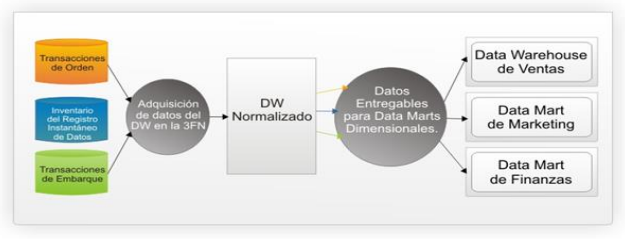
\includegraphics[width=9cm]{./IMAGENES/imgleydi2}
				\end{center}
			\end{figure}

La arquitectura que plantea Bill Inmon consta de las siguientes partes: \cite{robles1}

\begin{itemize}
		\item Fuente de la Información: Inicia el proceso de creación de un DW, conociendo la información que se necesita de todas las herramientas de las que se tengan acceso, ir a las necesidades de información que se necesitan con la finalidad de un resultado para crear un DW.

		\item Data Warehouse: La necesidad de normalizar toda la información extraída para ser almacenada en un DW, los cuales serán procesados y consultados por un DM.
		\item Data Marts: Se crean un subconjunto de los datos de un DW con el objetivo de responder a un determinado análisis o necesidad de una población, de un departamento en específico.
		\item Explotación de los datos: Se refiere a la manera de presentación de la información para ser consultada y analizada por las áreas. En cuanto a la arquitectura interna de un DW, Bill Inmon considera las siguientes características:

			\begin{itemize}
				\item Normalización: el DW debe ser basado y diseñado, conforme al diseño de las bases de datos transaccionales con las que se esté interactuando.
				\item Tercera Forma normal: la prioridad es que el modelo de datos esté construido en TFN con lo cual se tenga mayor relación entre los objetos de la base de datos.
			\end{itemize}

\end{itemize}

\subsection{La estructura del DataWarehouse}	
En cuanto a la estructura interna del DataWarehouse, para Inmon la prioridad es que el modelo de datos esté construido en tercera forma normal. Por dar una breve explicación de lo que esto significa, el proceso de normalización consiste en aplicar una serie de reglas o normas a la hora de establecer las relaciones entre los diferentes objetos dentro de la base de datos. Con este proceso de normalización se consiguen muchos beneficios, como evitar la redundancia de los datos, mantener su integridad referencial, facilitar el mantenimiento de las tablas y disminuir el tamaño de la base de datos. Sin embargo, a diferencia de los DataWarehouse desnormalizados, las consultas exigen el empleo de queries mucho más complejas, lo que dificulta el análisis directo de la información y el uso de las herramientas de reporting. De ahí, la necesidad de construir los DataMarts que, como ya comenté, están basados en modelos dimensionales de estrella o copo de nieve, diseños fácilmente explotables por estas herramientas de análisis de datos.\cite{estrella3}

			\begin{figure}[htb]
				\begin{center}
					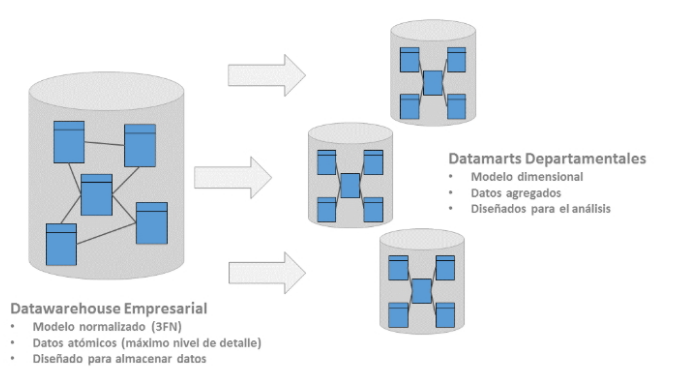
\includegraphics[width=9cm]{./IMAGENES/imgleydi3}
				\end{center}
			\end{figure}
%-------------------------------------------------
\subsection{METODOLOGIA SEGUN KIMBALL}	
La metodología se basa en lo que Kimball denomina Ciclo de Vida Dimensional del Negocio. Este ciclo de vida del proyecto de DW, está basado en cuatro principios básicos: 

\begin{itemize}
	\item Centrarse en el negocio: Hay que concentrarse en la identificación de los requerimientos del negocio y su valor asociado, y usar estos esfuerzos para desarrollar relaciones sólidas con el negocio, agudizando el análisis del mismo y la competencia consultiva de los implementadores. 
	\item Construir una infraestructura de información adecuada: Diseñaruna base de información única, integrada, fácil de usar, de alto rendimiento donde se reflejará la amplia gama de requerimientos de negocio identificados en la empresa. 
	\item Realizar entregas en incrementos significativos: crear el almacén de datos (DW) en incrementos entregables en plazos de 6 a 12 meses.
	\item Ofrecer la solución completa: proporcionar todos los elementos necesarios para entregar valor a los usuarios de negocios. 
\end{itemize}

La construcción de una solución de DW/BI (Datawarehouse/Business Intelligence) es sumamente compleja, y Kimball nos propone una metodología que nos ayuda a simplificar esa complejidad. Las tareas de esta metodología (ciclo de vida) se muestranen la figura 1.

				\begin{center}
					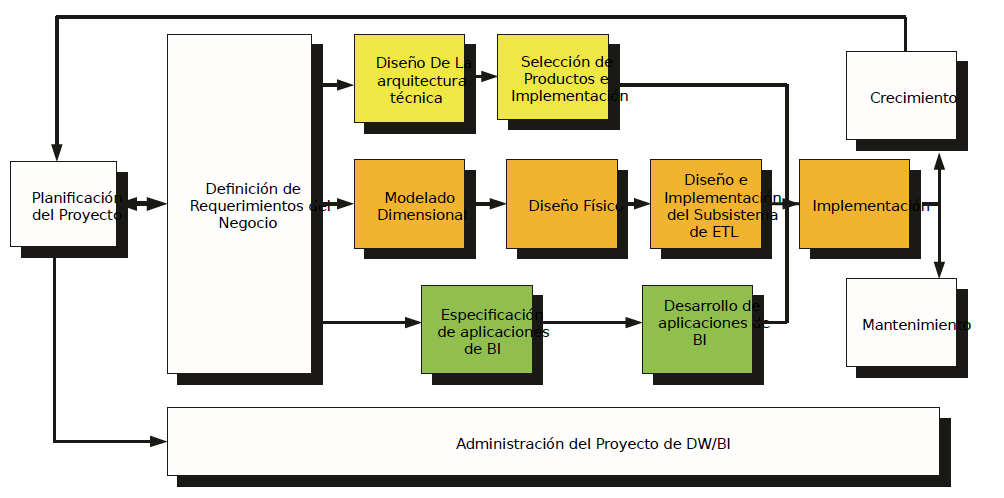
\includegraphics[width=8cm]{./IMAGENES/img01}
				\end{center}
				
Fig. 1: Tareas de la metodología de Kimball, denominada Business Dimensional Lifecycle 

De la figura 1, podemos observar dos cuestiones. Primero, hay que resaltar el rol central de la tarea de definición de requerimientos. Los requerimientos del negocio son el soporte inicial de las tareas subsiguientes. También tiene influencia en el plan de proyecto (nótese la doble fecha entre la caja de definición de requerimientos y la de planificación). En segundo lugar podemos ver tres rutas o caminos que se enfocan en tres diferentes áreas:

\begin{itemize}
	\item Tecnología (Camino Superior). Implica tareas relacionadas con software específico, por ejemplo, Microsoft SQL Analysis Services.
	\item Datos (Camino del medio). En la misma diseñaremos e implementaremos el modelo dimensional, y desarrollaremos el subsistema de Extracción, Transformación y Carga (Extract, Transformation, and Load - ETL) para cargar el DW.
	\item Aplicaciones de Inteligencia de Negocios (Camino Inferior). En esta ruta se encuentran tareas en las que diseñamos y desarrollamos las aplicaciones de negocios para los usuarios finales.
\end{itemize}

Estas rutas se combinan cuando se instala finalmente el sistema.
En la parte de debajo de la figura se muestra la actividad general de administración del proyecto. A continuación describiremos cada una de las tareas.\cite{estrella7}

4.4.1. Planificación

En este proceso se determina el propósito del proyecto de DW/BI, sus objetivos específicos y el alcance del mismo, los principales riesgos y una aproximación inicial a las necesidades de información.
En la visión de programas y proyectos de Kimball, Proyecto, se refiere a una iteración simple del KLC (Kimball Life Cycle), desde el lanzamiento hasta el despliegue.
Esta tarea incluye las siguientes acciones típicas de un plan de proyecto:

\begin{itemize}
	\item Definir el alcance (entender los requerimientos del negocio.
	\item Identificar las tareas.
	\item Programar las tareas.
	\item Planificar el uso de los recursos.
	\item Asignar la carga de trabajo a los recursos
	\item Elaboración de un documento final que representa un plan del proyecto.
\end{itemize}
Además en esta parte definimos cómo realizar la administración o gestión de esta subfase que es todo un proyecto en si mismo, con las siguientes actividades: 

\begin{itemize}
	\item Monitoreo del estado de los procesos y actividades.
	\item Rastreo de problemas.
	\item Desarrollo de un plan de comunicación comprensiva que direccione la empresa y las áreas de TI.
\end{itemize}

4.4.2. Análisis de requerimientos:
La definición de los requerimientos es en gran medida un proceso de entrevistar al personal de negocio y técnico, pero siempre conviene tener un poco de preparación previa. Se debe aprender tanto como se pueda sobre el negocio, los competidores, la industria y los clientes del mismo. Hay que leer todos los informes posibles de la organización; rastrear los documentos de estrategia interna; entrevistar a los empleados, analizar lo que se dice en la prensa acerca de la organización, la competencia y la industria. Se deben conocer los términos y la terminología del negocio. \cite{estrella5}

A partir de las entrevistas, podemos identificar temas analíticos y procesos de negocio. Los temas analíticos agrupan requerimientos
comunes en un tema común (ver tabla 1).
	            \begin{center}
					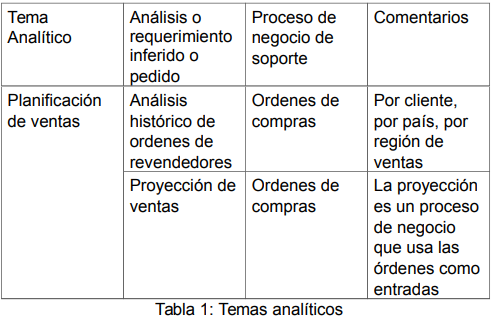
\includegraphics[width=9cm]{./IMAGENES/img02}
				\end{center}

Por otra parte, a partir del análisis se puede construir una herramienta de la metodología denominada matriz de procesos/dimensiones.
Una dimensión es una forma o vista o criterio por medio de cual se pueden sumariar, cruzar o cortar datos numéricos a analizar, datos que se denominan medidas.\cite{estrella8}
Esta matriz tiene en sus filas los procesos de negocio identificados,
y en las columnas, las dimensiones identificadas.
Un ejemplo de esta matriz se puede observar en la tabla 2. Cada X en la intersección de las filas y columnas significa que en el proceso de negocio de la fila seleccionada se identifican las dimensiones propuestas. 
                 \begin{center}
					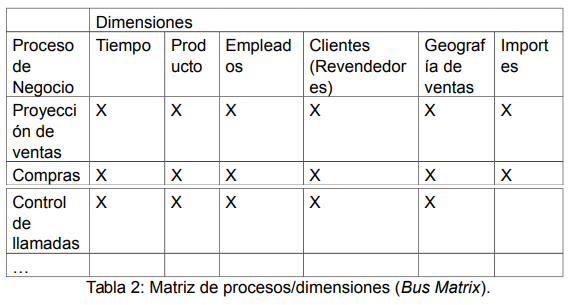
\includegraphics[width=9cm]{./IMAGENES/img03}
				\end{center}
Finalmente se busca priorizar los requerimientos o procesos de negocios más críticos. 

4.4.3. Modelado Dimensional
La creación de un modelo dimensional es un proceso dinámico y altamente iterativo. Un esquema general se puede ver en la figura 2. 
\begin{center}
	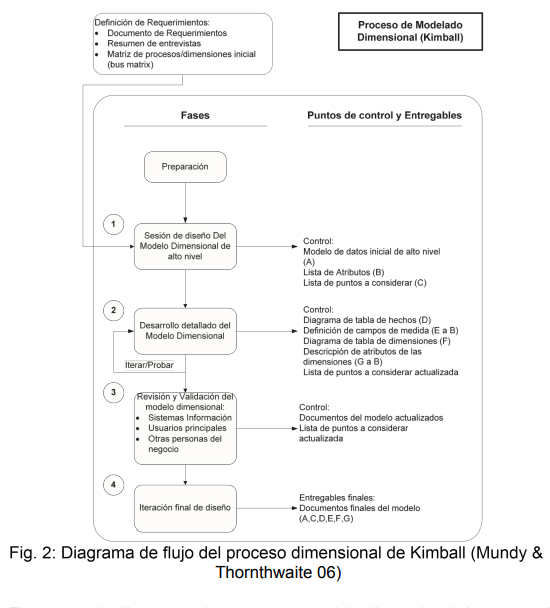
\includegraphics[width=9cm]{./IMAGENES/img04}
\end{center}

El proceso de diseño comienza con un modelo dimensional de alto nivel obtenido a partir de los procesos priorizados de la matriz descrita en el punto anterior.
El proceso iterativo consiste en cuatro pasos:

\begin{itemize}
	\item Elegir el proceso de negocio: El primer paso es elegir el área a modelizar. 
    \item Establecer el nivel de granularidad: La granularidad significa especificar el nivel de detalle.
    \item Elegir las dimensiones: Las dimensiones surgen naturalmente de las discusiones del equipo, y facilitadas por la elección del nivel de granularidad y de la matriz de procesos/dimensiones. 
    \item Identificar medidas y las tablas de hechos: El último paso consiste en identificar las medidas que surgen de los procesos de negocios.
\end{itemize}

%-------------------------------------------------
\subsection{IMPLEMENTACIONES DE KIMBALL}

Implementación Datawarehouse con Metodología Kimball
La inteligencia de negocios (BI) es un conjunto de metodologías, aplicaciones y tecnologías que aporta a empresas y organizaciones información privilegiada y debidamente estructurada, que sirve de soporte a la toma de decisiones.

Permite obtener datos relacionados con las alternativas de ingreso a nuevos mercados, ofertas de productos, eliminación de islas de información, controles financieros, optimización de costos, planificación de la producción , análisis de perfiles de clientes, rentabilidad de un producto, etc., para analizarlos y convertirlos en conocimiento.\cite{estrella4}

En la práctica, la inteligencia de negocios es un factor determinante para el éxito y su implementación  no sería nada fácil, si no contáramos con un instrumento como la Metodología Kimball, para la construcción de un almacén de datos (Datawarehouse)  circunscrito al ámbito de la empresa, de manera integrada y permanente (pero variable) en el tiempo.

Producto de nuestra experiencia en el diseño de Datamart (base de datos departamentales) para un sistema de datawarehouse basado en la Metodología Kimball, hemos rescatado y exponemos en el  siguiente artículo algunos apuntes y sugerencias que consideramos de relevancia para aquellos que deseen implementar o explorar soluciones de esta naturaleza:\cite{estrella6}

\begin{itemize}
	\item Una vez seleccionado el proceso al que se va a diseñar una solución OLAP (base de datos orientada al procesamiento analítico) es necesario efectuar un análisis y crear un diagrama OLTP (base de datos orientada al procesamiento de transacciones) de cada modelo implicado.
    \item Identificar correctamente el “Grano” en el que está la información, es decir el nivel mínimo de detalle para el que se puede obtener una medida determinada o identificar determinado evento que ha ocurrido.
    \item Efectuar un análisis y crear un modelo OLAP que especifique las tablas de dimensión y de hechos resultantes, de preferencia, planteada en una “Topología Estrella”. En este modelo de datos debe converger toda la información de las distintas fuentes identificadas.
    \item Es conveniente se nombre las tablas con el prefijo adecuado según la naturaleza de cada tipo de tabla OLAP (DIM, FACT). Los nombres para las tablas DIM (dimensiones) deben acabar en singular y los nombres de las tablas FACT (hechos) en plural.
    \item Es preciso crear llaves subrogadas para todas las dimensiones, es decir una nueva llave, un valor correlativo único diferente a la llave natural que viene del registro en el sistema fuente OLTP, que también se conserva.
    \item En la tabla de hechos deben ir todos aquellos eventos o transacciones que ocurren, como ventas, pagos, compras, logs, etc.
    \item Toda tabla del DWH debe contar con un timestamp o de registro que permita determinar en qué fecha, hora, minuto y segundo se creó determinado registro en la base de datos.
    \item En cada dimensión se deben crear los registros default para los casos en que la información no esté disponible, no aplique o simplemente no exista y así poder distinguir estos escenarios en los hechos
    \item Es necesario tener muy en consideración el cómo manejar los casos de Null, sugiriendo evaluar la siguientes alternativas.
    \item Contar con una dimensión “Tiempo” con los pre-cálculos de fecha ya realizados y así ahorrarle esta tarea de procesamiento a quienes exploten la información del DWH. La dimensión tiempo podría tener la siguiente información:
    
    \begin{itemize}
	\item Mes, año, día del mes.
	\item La fecha competa incluyendo el nombre del día.
	\item El nombre corto del día, el día de la semana en números.
	\item El nombre corto correspondiente al día de la semana.
	\item Flag fin de semana.
	\item Flag si es laborable o no, es decir si son días en los cuales se trabaja.
	\item El día del mes en número.
	\item El día del año en número.
	\item La semana del mes en número.
	\item El nombre de la semana del mes.
	\item La semana del año.
	\item El número de días que tiene el mes.
	\item La fecha del fin del mes.
	\item El mes del año.
	\item El nombre del mes del año.
	\item El nombre corto del mes del año.
	\item La combinación del año y el mes en números.
	\item El trimestre del año al que corresponde una fecha.
	\item El nombre del trimestre del año al que corresponde una fecha.
	\item La fecha de finalización del trimestre.
	\item El semestre del año al que corresponde una fecha.
	\item Flag su es cierre de mes.
    \end{itemize}
\end{itemize}

%-------------------------------------------------
\subsection{ARQUITECTURA SEGUN KIMBALL}

Ralph Kimball, plantea la idea de un enfoque dimensional para el diseño de un DW, y afirma que la unión de todos los DM de una organización constituye el DW corporativo, a lo cual se le conoce como el enfoque bottom-up.\\

Su filosofía se centra en que, en la mayoría de las organizaciones, la construcción de un datawarehouse se origina por el interés y esfuerzo de un departamento. Es por esto por lo que en su primera versión este datawarehouse no es más que un datamart departamental.\\

El esquema de arquitectura en base a los fundamentos de Ralph Kimball sería el de la siguiente imagen:

     				\begin{center}
					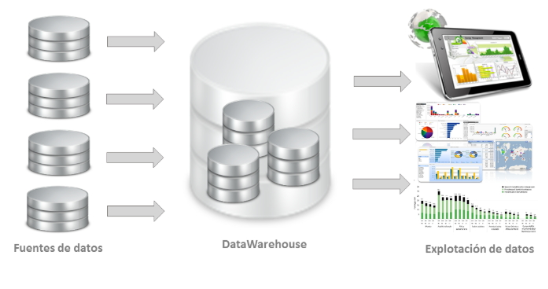
\includegraphics[width=9cm]{./IMAGENES/arquitectura}
				\end{center}

 

%-------------------------------------------------

\subsection{COMPARACIÓN DE METODOLOGIAS}	

\begin{itemize}
\item Mientras Kimball utiliza modelos dimensionales para los datos, Inmon utiliza modelos dimensionales solo para los marts de datos. Ahora desde una perspectiva arquitectónica, Kimball propone que no es necesario separar los data marts del almacén de datos dimensionales existente. Mientras que en el caso de Inmon, se utiliza los data marts derivados de los data warehouse para separarlos físicamente del data warehouse como unidades separadas.
\item Con el enfoque de Kimball, esté puede identificar el proceso comercial clave y las soluciones comerciales posteriores que se deben proporcionar con el almacén de datos. Mientras que el enfoque de Inmon cree en la construcción de un almacén de datos con el modelo de datos corporativos.
\item El enfoque de Kimball utiliza modelos dimensionales como el esquema de estrella y copo de nieve con el fin de organizar los datos en varios datos clasificados de negocios, a fin de habilitar rápidamente los procesos de negocios. Inmon, por otro lado, considera el requisito general de datos corporativos y, como tal, utiliza la técnica de modelado ER. 
\item Kimball se centra en proporcionar sistemas analíticos a los que se pueda acceder directamente desde el almacén de datos. Mientras que en el caso de Inmon, la arquitectura está diseñada de tal manera que el sistema analítico solo puede acceder a los datos del almacén de datos a través de los data marts.
\item Inmon trabaja con el modelo de datos normalizado, mientras que Kimball prefiere el modelo de datos desnormalizado y, como tal, se encuentran modelos de datos redundantes presentes en la arquitectura de Kimball. El diseño y la arquitectura de Inmon pueden ser complejos, pero los almacenes de datos basados en Kimball son más fáciles de diseñar e implementar.
\item Los recursos involucrados necesitan saber cómo trabajar con el modelado ER, sin la necesidad de desacoplarlos en varios mercados de datos. Se necesita la integración de datos en toda la empresa con el almacén de datos basado en Inmon. Mientras que con el almacén de datos basado en Kimball, el requisito de integración de datos se centra en el área comercial individual.\cite{torres}
\end{itemize}

%-----------------------------------------------------------------
\section{Conclusiones}

\begin{itemize}
\item Mantener un almacen de datos basado en Inmmon es fácil debido a que se puede desacoplar las tareas de mantenimiento en diversas actividades de mamtenimiento de data mart. En el caso del diseño basado en la metodología de Kimball, referente al mantenimiento es dificil porque puede hacer datos redundantes.
\item La implementación de un almacen de datos basados en Inmmon puede generar altos costos iniciales. Kimball, por otro lado, incurre en un bajo costo inicial y el costo sigue siendo el mismo para las fases posteriores.
\item Kimball requiere un equipo generalista para implementar esta metodología, pero cuando se implementa un almacen de datos basado en Inmon, se necesita un equipo especializado.
\end{itemize}

%-----------------------------------------------------------------
\section{Recomendaciones}

\begin{itemize}
\item La metodología Kimbal utiliza una implementación de una cantidad de tiempo relativamente menor,  mientras que Inmmon es un método que lleva bastante tiempo implementarlo.
\item Se debe tener en cuenta que los almacenes de datos que estan basados en Kimball se puede configurar de una manera rapida, pero la arquitectura de almacen de datos que se encuentra basada en Inmon requiere un tiempo mayor de inicio.
\end{itemize}

% Bibliografia.
%-----------------------------------------------------------------

\bibliographystyle{apalike}

\bibliography{Bibliografia}

\end{document}
